\documentclass{beamer}
\usepackage{../tut-slides}
\usepackage{../mathoperatorsAuD}

\usepackage{lmodern}
\usepackage{amsmath,amssymb}
\usepackage{wasysym}
\usepackage{stmaryrd}
\usepackage{enumerate}
%\usepackage[inline]{enumitem} 		%customize label
%\newcommand{\labelitemi}{\raisebox{1pt}{\scalebox{.9}{$\blacktriangleright$}}}
%\newcommand{\labelitemii}{$\vartriangleright$}
%\newcommand{\labelitemiii}{--}
\setbeamertemplate{itemize item}{\raisebox{1pt}{\scalebox{.9}{$\blacktriangleright$}}}
\setbeamertemplate{itemize subitem}{$\vartriangleright$}

\usepackage{booktabs}
\usepackage{tabularx}
\usepackage{tabu}
\newcommand*\head{\rowfont{\bfseries}}
\newcommand*{\tw}{\rowfont{\ttfamily}}
\renewcommand{\tabularxcolumn}[1]{>{\hspace{0pt}}m{#1}}
\usepackage{multirow}

\usepackage{cancel}

\usepackage{empheq}
\newcommand*\widefbox[1]{\fbox{\hspace{2em} #1 \hspace{2em}}}

\usepackage{tcolorbox}
\newtcolorbox{mymathbox}[1][]{colback=white, sharp corners, #1}

\usepackage{xcolor}
\usepackage{listings}
\lstset{numbers=left, 
	numberstyle=\tiny, 
	breaklines=true,
	backgroundcolor=\color{cdgray!20},
	numbersep=5pt,
	language=C,
	tabsize=2,
	basicstyle=\footnotesize\ttfamily,
	showstringspaces=false} 

\usepackage{MnSymbol}

\newcommand{\col}[1]{\textcolor{cdpurple}{#1}}
\newcolumntype{R}[1]{>{\centering\arraybackslash}p{#1}}
\usepackage{tabularx}
\renewcommand{\tabularxcolumn}[1]{m{#1}}

\usepackage{cancel}

\usepackage{qtree}
\usepackage[edges]{forest}

\usepackage[normalem]{ulem}
\newcommand{\person}[1]{\textsc{#1}}
\newcommand{\begriff}[1]{\textbf{#1}}

\usepackage{ragged2e}
\usepackage{caption}
\setbeamerfont{caption}{size=\footnotesize}


\begin{document}	
	\title{Algorithmen und Datenstrukturen}
	\subtitle{Der Dijkstra-Algorithmus}
	\author{Eric Kunze}
	\email{eric.kunze@mailbox.tu-dresden.de}
	\city{TU Dresden}
%	\institute{Lehrstuhl für Grundlagen der Programmierung}
	\titlegraphic{\includegraphics[width=2cm]{../TUD-white.pdf}}
	\date{03.03.2020}

	\maketitle

%%%%%%%%%%%%%%%%%%%%%%%%%%%%%%%%%%%%%%%%%%%%%%%%%%%%%%%%%%%%%%%%%%%%%%%%%%%%%%%%%%%

%\section{Algorithmus von \person{Dijkstra}}

\begin{frame} \frametitle{Setting \cite{vogler}}
	\textbf{gegeben:} 
	\begin{itemize}
		\item gerichteter, gewichteter Graph $G = (V,E,c)$ mit
		\begin{itemize}
			\item $V = \menge{1, \dots, n}$ 
			\item $c(v) \ge 0$ für alle $v \in V$ (nichtnegative Kantengewichte)
		\end{itemize}
		\item Startknoten $s$ (\textit{Quelle})
	\end{itemize}
	\textbf{Ziel:} 
		\begin{itemize}
			\item kürzeste Entfernung von $s$ nach $v$ für alle $v \in V$ 
		\end{itemize}
	\textbf{Idee:}
		\begin{itemize}
			\item Wir kennen einen kürzesten Weg $p$ von $s$ nach $v$.
			\item Verlängerung von $p$ um eine Kante $(v,v')$
			\item Wir erhalten einen kürzesten Weg von $s$ nach $v'$.
		\end{itemize}
\end{frame}

\begin{frame} \frametitle{Optimalitätseigenschaft}
	\begin{theorem}
		Für jeden kürzesten Weg $p = (v_0, v_1, \dots, v_k)$ von $v_0$ nach $v_k$ ist jeder Teilweg $(v_i, \dots, v_j)$ mit $1 \le i < j \le k$ auch ein kürzester Weg von $v_i$ nach $v_j$.
	\end{theorem}
	\begin{justify}
		\footnotesize
		\textbf{Beweis} (nach \cite{buesing})\textbf{.} Sei $p$ wie oben ein kürzester Weg. Angenommen es gäbe einen Teilweg $(u, \dots, v)$, der kein kürzester Weg ist. Dann gibt es also einen kür"-zer"-en Weg $(u, w_1, \dots, w_\ell, v)$ von $u$ nach $v$. Dann wäre aber auch der Weg $p' = (v_1, \dots, u, w_1, \dots, w_\ell, v, \dots, v_k)$ von $v_1$ nach $v_k$ kürzer als $p$ im Widerspruch zur Optimalität von $p$. Also muss auch der Weg $(u, \dots, v)$ optimal sein. \qed
	\end{justify}

	\centering
	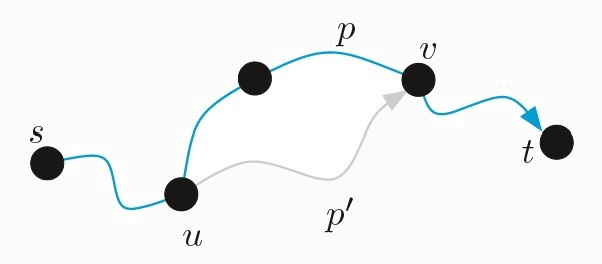
\includegraphics[width=10em]{./optimaleWege.jpg}
	\captionof{figure}{Teilwege von optimalen Wegen sind wieder optimal. \cite{buesing}}
\end{frame}

\begin{frame} \frametitle{Der Algorithmus \cite{martinovic}}
	\small
	\textbf{Notation.}
	\begin{itemize}
		\item $M$ \dots Menge der Knoten, zu der ein kürzester Weg bekannt ist
		\item $p(v_k)$ \dots Vorgänger von $v_k$ auf dem kürzesten Weg nach $v_k$
		\item $d(v_k)$ \dots Länge des (bisher) kürzesten Weges zu $v_k$
	\end{itemize}

	\textbf{Initialisierung.}
	\begin{itemize}
		\item $M = \menge{s}$
		\item $d(s) = 0$
		\item für $v \neq s$ setze
		\begin{equation*}
			p(v) \defeq \begin{cases}
			s & \text{für } (s,v) \in E \\ 0 & \text{für } (s,v) \notin E
			\end{cases} 
			\qquad
			d(v) \defeq \begin{cases}
			c(s,v) & \text{für } (s,v) \in E \\ +\infty & \text{für } (s,v) \notin E
			\end{cases}
		\end{equation*}
	\end{itemize}
\end{frame}

\begin{frame} \frametitle{Der Algorithmus \cite{martinovic}}
	\begin{enumerate}
		\item Bestimme $u \notin M$ mit $d(u) = \min\menge{d(v) : v \notin M}$. 
		\begin{itemize}
			\item Falls $d(u) = +\infty$, dann \texttt{STOP} (kein neuer Weg möglich)
			\item Andernfalls setze $M \defeq M \cup \menge{u}$
		\end{itemize}
		\item Für alle $v \notin M$ mit $(u,v) \in E$:  \\
		falls $d(v) > d(u) + c(u,v)$ (also ein kürzerer Weg ist gefunden), \\
		dann setze $d(v) = d(u) + c(u,v)$ und $p(v) = u$
		\item Falls $M \neq V$, gehe zu Schritt 1. Sonst \texttt{STOP}.
	\end{enumerate}
\end{frame}

\begin{frame} \frametitle{Beispiel}
	Wir notieren die notwendigen Informationen als Tripel
	\begin{equation*}
	\small
	\setlength{\arraycolsep}{1pt}
	\begin{array}{rcccccc}
		\Big( & \text{Knotennummer} &,& \text{Entfernung von der Quelle} &,& \text{Vorgängerknoten} & \Big) \\
		= \Big( & v_k &,& d(v_k) &,& p(v_k) & \Big)
	\end{array}		
	\end{equation*}
	
	\centering
	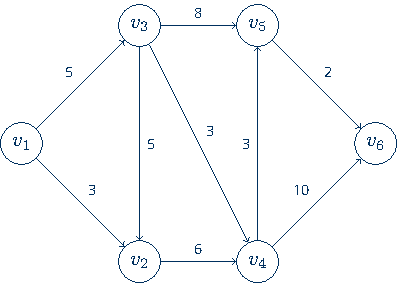
\includegraphics[height=13em]{./beispiel.pdf}
	\captionof{figure}{Graph $G = (V,E,c)$}
\end{frame}

\begin{frame} \frametitle{Beispiel}
	\centering
	\renewcommand{\arraystretch}{1.5}
	\begin{tabular}{l|l}
		\hline
		gewählt & Menge der Randknoten \\ \hline
		$(v_1,0,-)$ & $\menge{\underline{(v_2,\mathbf{3},v_1)}, (v_3, 5, v_1)}$ \\
		$(v_2, 3, v_1)$ & $\menge{\underline{(v_3, \mathbf{5}, v_1)}, (v_4, 9, v_2)}$ \\
		$(v_3,5,v_1)$ & $\menge{\underline{(v_4, \alert{\mathbf{8}}, \alert{v_3})}, (v_5, 13, v_3)}$ \\
		$(v_4, 8, v_3)$ & $\menge{\underline{(v_5, \alert{\mathbf{11}}, \alert{v_4})}, (v_6, 18, v_4)}$ \\
		$(v_5, 11, v_4)$ & $\menge{\underline{(v_6, \alert{\mathbf{13}}, \alert{v_5})}}$ \\
		$(v_6, 13, v_5)$ & $\emptyset$ \\ \hline
	\end{tabular}
\end{frame}

\begin{frame} \frametitle{Rekonstruktion des kürzesten Weges}
	Wir betrachten beispielhaft den Weg von $v_1$ nach $v_5$.
	\begin{itemize}
		\item Es ist $d(v_5) = 11$, d.h. der kürzeste Weg von $v_1$ zu $v_5$ ist $11$~Einheiten lang.
		\item Es gilt $p(v_5) = v_4$. Wir betrachten weiter die Vorgänger-Funktion:
		\begin{equation*}
		p(v_5) = v_4 \quad \leftarrow \quad p(v_4) = v_3 \quad \leftarrow \quad p(v_3) = v_1
		\end{equation*}
		Somit ist der kürzeste Weg von $v_1$ zu $v_5$ also gegeben durch
		\begin{equation*}
		v_1 \to v_3 \to v_4 \to v_5
		\end{equation*}
	\end{itemize}
\end{frame}

\begin{frame} \frametitle{Eine andere Art der Dokumentation}
	\centering
	\begin{tabular}{r|cccccc}
		\hline
		$p =$ & 0 & $v_1$ & $v_1$ & \cancel{$v_2$} \alert{$v_3$} & \cancel{$v_3$} \alert{$v_4$} & \cancel{$v_4$} \alert{$v_5$} \\ \hline
		& $v_1$ & $v_2$ & $v_3$ & $v_4$ & $v_5$ & $v_6$ \\ \hline
		$d =$ & \uline{0} & $\infty$ & $\infty$ & $\infty$ & $\infty$ & $\infty$ \\
		&  & \uline{3} & 5 & $\infty$ & $\infty$ & $\infty$  \\
		&          &  & \uline{5}  & 9 & $\infty$ & $\infty$  \\
		&          &  &            & \uline{\alert{8}} & 13                 & $\infty$  \\
		&          &   &           &                   & \uline{\alert{11}} & 18  \\
		&          &   &           &                   &                    & \uline{\alert{13}} \\
		\hline
	\end{tabular}
\end{frame}

\begin{frame} \frametitle{Literatur}
%	\nocite{*}	
	\bibliographystyle{abbrvdin} 
	% alternativ:  abbrvdin alphadin natdin plaindin unsrtdin
	\bibliography{literatur}
\end{frame}

%%%%%%%%%%%%%%%%%%%%%%%%%%%%%%%%%%%%%%%%%%%%%%%%%%%%%%%%%%%%%%%%%%%%%%%%%%%%%%%%%%%


\end{document}